\documentclass[manuscript,screen,review,anonymous]{acmart}

\usepackage{graphicx}
\usepackage{hyperref}
\usepackage{url}
\usepackage{array}
\setlength{\headheight}{21pt}

% Conference information
\acmConference[ASSETS '26]{The 28th International ACM SIGACCESS Conference on Computers and Accessibility}{October 26--28, 2026}{Athens, Greece}

\acmYear{2026}
\copyrightyear{2026}

%Porto, Portugal, why does this say greece? why does the pdf say new york

\begin{document}

\title{ACCESS KNOB: Parametric Design of 3D-Printable Accessible Synthesizer Controls for Users with Reduced Hand Strength}

% Anonymized for double-blind review
\author{Anonymized Author(s)}
\email{anonymous@example.com}
\affiliation{%
  \institution{Anonymized Institution}
  \city{Anonymized City}
  \state{Anonymized State}
  \country{Anonymized Country}
}

% Author details for final camera-ready version:
% \author{Dillon Simeone}
% \authornote{Deaf Lead Design Engineer - Universal Music Design}
% \email{dillonsimeone@gmail.com}
% \affiliation{%
%   \institution{CymaSpace / Universal Music Design}
%   \city{Portland}
%   \state{Oregon}
%   \country{USA}
% }
%
% \author{Doga Cavdir}
% \email{cavdir@ccrma.stanford.edu}
% \affiliation{%
%   \institution{IT University of Copenhagen / Universal Music Design / Affective Interactions and Relations Lab}
%   \city{Copenhagen}
%   \country{Denmark}
% }

% \author{Tracy Held}
% \email{tracyheld@gmail.com}
% \affiliation{%
%   \institution{Confluence Recording Co./ Universal Music Design}
%   \city{Portland}
%   \state{Oregon}
%   \country{USA}
% }

% \author{Shawn Trail}
% \email{shawntrail@gmail.com}
% \affiliation{%
%   \institution{Confluence Recording Co./ Universal Music Design}
%   \city{Portland}
%   \state{Oregon}
%   \country{USA}
% }

\begin{abstract}
Synthesizers and electronic musical instruments are popular tools for creating contemporary music, offering versatile expressions of music compositions that easily transfer to electronic media platforms. While these tools increase the accessibility of music production to broader populations, particularly by reducing barriers for recording and distributing music while also at times lowering the overhead towards instrumental proficiency, the physical design of the instruments present significant accessibility barriers for users with motor impairments affecting grip strength and fine motor control. These barriers unnecessarily deter musicians bearing these impairments from creating music. To address this, the ACCESS KNOB, an open-source parametric web tool for generating customizable 3D-printable knobs, will  make it possible to create replacement knobs for synthesizers and electronic musical instruments that can be operated with reduced hand strength and sensation. 
\end{abstract}

\begin{CCSXML}
<ccs2012>
<concept>
<concept_id>10003120.10003121.10003124</concept_id>
<concept_desc>Human-centered computing~Accessibility technologies</concept_desc>
<concept_significance>500</concept_significance>
</concept>
<concept>
<concept_id>10003120.10003121.10003125</concept_id>
<concept_desc>Human-centered computing~Accessibility design and evaluation methods</concept_desc>
<concept_significance>300</concept_significance>
</concept>
<concept>
<concept_id>10010405.10010455</concept_id>
<concept_desc>Applied computing~Sound and music computing</concept_desc>
<concept_significance>500</concept_significance>
</concept>
</ccs2012>
\end{CCSXML}

\ccsdesc[500]{Human-centered computing~Accessibility technologies}
\ccsdesc[300]{Human-centered computing~Accessibility design and evaluation methods}
\ccsdesc[500]{Applied computing~Sound and music computing}

\keywords{accessibility, assistive technology, parametric design, 3D printing, synthesizers, motor impairments, universal design, music technology}

\maketitle

\section{Introduction}

Musical expression through synthesizers and electronic instruments requires precise tactile control of numerous parameters, such as knobs, faders, and buttons. For users with motor impairment, reduced grip strength, or diminished hand sensation, these standard interface controls can present insurmountable barriers to the usability of these tools that limit full access to music expression. The typical synthesizer knob—small in diameter, smooth or minimally textured, and requiring precision grip and fine motor control—excludes a significant population of potential users. \cite{vamvakousis2016dmi}

This work was commissioned by a retired IT professional and avid synthesizer collector who, due to dialysis-dependent kidney failure, had progressively lost hand strength and sensation. This disability grew to the point where his wall of rare synthesizers, accumulated over decades, had become largely unplayable. Workarounds failed to produce the nuanced, expressive control integral to synthesizer performance.

Although many people will experience decreased fine motor skills and grip strength decline through age or injury, standard synthesizers and electronic instruments favor smaller knob designs with no mainstream alternatives. \cite{larsen2016prospects}

ACCESS KNOB leverages the increased availability of 3D printers and laser cutters \cite{nime2026_92}
to allow musicians to generate customized 3D-printable replacement knobs using a parametric web-based tool. Building on the principles of Universal Music Design (UMD) (\cite{hergert2024gestolumina}, \cite{cavdir2025sonic}), ACCESS KNOB addresses motor accessibility while maintaining applicability for all users. A video demo of this platform is available \href{https://www.youtube.com/watch?v=cEG93wy7U9o}{here}.

We contribute: (1) documentation of a parametric design system for accessible synthesizer controls informed by lived disability experience; (2) an engineering evaluation of the parametric design space, physical print tolerances, and mechanical torque advantages; (3) discussion of extensibility to other instrument types and assistive device domains; and (4) reflection on open-source distribution as an accessibility strategy \cite{strail2014_nime}.

\section{Related Work} %shawnpaper

Research in accessibility-focused Digital Musical Instruments (DMIs) has historically prioritized eye-tracking, occupational therapy frameworks, rapid prototyping of bespoke instruments, or entirely novel interfaces to support musicians with diverse motor and cognitive impairments \cite{frid2019accessible, mcmillan2023designing, mccloskey2015accessibility, payne2020eye, holland2020expanding}. However, these approaches focus on creating new instruments rather than retrofitting existing commercial hardware, leaving classic physical synthesizers largely inaccessible. Parametric and generative design frameworks address this by enabling personalized, custom-fit physical adaptations, such as non-invasive mappable gesture sensing \cite{strail2012nime} and custom 3D-printed orthopedic grips or pneumatic controls with variable activation forces \cite{tandon2023parametric, santos2023parametric, desai20153dprinting}. Generative systems further democratize fabrication by exploring design spaces algorithmically, removing manual CAD editing bottlenecks \cite{hofmann2020living}. ACCES KNOB builds on this by utilizing a mutation engine to generate customizable variant batches, ensuring direct user agency in selecting ergonomic shapes.

ACCESS KNOB integrates and promotes UMD's ethos of sonic agency \cite{labelle2018sonic} to increase accessibility of music technology that historically excluded DHH musicians and musicians with motor disabilities. These frameworks emphasize multimodal, cross-disability design by integrating visual, auditory, and haptic feedback channels \cite{breteche2019deaf, cavdir2022embodied}. %these are redundant, are there more cannonical examples? 

This is particularly relevant for DHH musicians who utilize vibrotactile interfaces for sensory reinforcement \cite{cavdir2022touch, cavdir2020felt}. Given that vestibular variations in DHH populations can affect motor coordination \cite{wink2018balance, erkilicc2011conceptual}, our parametric customizer combines tactile shapes, voice/facial inputs, and auditory/haptic feedback to unify motor and sensory accessibility.

\section{System Description}

ACCESS KNOB is a browser-based parametric design tool built using JavaScript, Three.js for 3D visualization, and a custom geometry engine for procedural knob generation. The interface provides a 3D real-time preview, parameter sliders, export options, and a mutation engine for the exploration of generative designs.

\subsection{Parametric Controls}
% Keep standard parametric inputs
Users adjust the following parameters via sliders and numerical inputs (Table~\ref{tab:knobparameters}).

%\textbf{Shape}: The cross-sectional profile, including circular, square, hexagonal, triangular, pentagonal, octagonal, star, or gear geometries. Shape-coding aids users with low vision in distinguishing knob functions by touch and sight (Figure~\ref{fig:profiles}), extending tactile design methods for accessible physical graphics \cite{manenti2024accessibility}.

%\textbf{Outer Diameter}: Range 15mm--50mm. Larger diameters reduce required grip force by increasing mechanical advantage. Default 35mm based on ergonomic mechanical advantage recommendations.

%\textbf{Height}: Range 10mm--40mm. Taller knobs provide greater surface area for palm-dragging techniques and accommodate varied grip strategies.

%\textbf{Taper}: Angle 0\%--70\%. Tapering provides ergonomic grip variation and visual/tactile distinction between knobs.

%\textbf{Groove Depth}: Range 1mm--5mm. Deep grooves increase friction and provide tactile landmarks for users with reduced sensation.

%\textbf{Groove Width}: Range 1mm--5mm. Wider grooves accommodate users with limited finger dexterity.

%\textbf{Groove Count}: Range 4--12. Higher counts provide finer tactile resolution; lower counts increase individual groove prominence.

%\textbf{Groove Profile}: Square, rounded, or V-shaped. Profile affects grip friction and tactile feel.

%\textbf{Bore Diameter}: Range 4mm--10mm. Matches shaft diameter of target synthesizer. Knob database provides common values for popular synthesizers.

%\textbf{Slot Depth}: D-shaft slot depth for rotational locking, 0mm--3mm.

%\textbf{Clearance}: Bore fit tolerance, 0mm--0.5mm, adjustable for printer precision and friction-fit preference.

%\textbf{Set Screw}: Toggle and position (top/side). Enables secure mechanical fastening without requiring friction fit.

\begin{table}[t]
\centering
\caption{Primary parametric knob design parameters.}
\label{tab:knobparameters}
\begin{tabular}{|>{\raggedright\arraybackslash}p{2.6cm}|>{\raggedright\arraybackslash}p{2.6cm}|p{6.6cm}|}
\hline
\textbf{Parameter} & \textbf{Range / Options} & \textbf{Purpose} \\
\hline
Shape & Circular, square, hexagonal, triangular, pentagonal, octagonal, star, gear &
Shape-coding enables tactile and visual differentiation of control functions, supporting users with low vision through recognizable profiles (Fig.~\ref{fig:profiles}) \cite{manenti2024accessibility}. \\
\hline
Outer Diameter & 15--50 mm (default: 35 mm) &
Larger diameters increase mechanical advantage and reduce the grip force required for rotation. \\
\hline
Height & 10--40 mm &
Taller knobs increase graspable surface area, supporting palm-dragging and diverse grip strategies. \\
\hline
Taper & 0--70\% Angle&
Provides ergonomic grip variation and improves visual and tactile distinction between controls. \\
\hline
Groove Profile & Square, rounded, V-shaped &
Affects grip friction, tactile feel, and rotational control. \\
\hline
Bore Diameter & 4--10 mm &
Matches the shaft diameter of the target synthesizer. A knob database provides common dimensions for popular synthesizers. \\
\hline
Slot Depth & 0--3 mm &
Controls D-shaft slot depth for secure rotational locking. \\
\hline
Clearance & 0--0.5 mm &
Adjusts bore fit tolerance for printer precision and preferred friction fit. \\
\hline
Set Screw & Enabled/Disabled; Top or Side &
Provides secure mechanical fastening independent of friction fit. \\
\hline
\end{tabular}
\end{table}

\begin{figure}[ht]
  \centering
  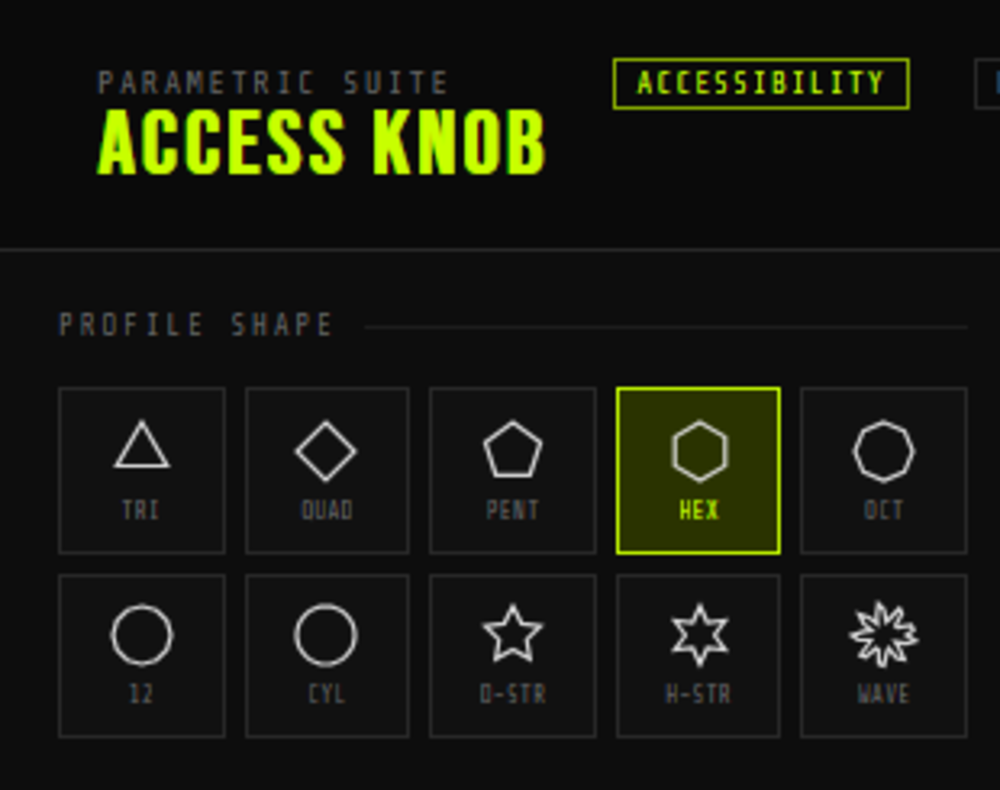
\includegraphics[width=0.9\columnwidth]{ProfileShapes.png}
  \Description{A diagram showcasing various cross-sectional geometric profiles for the knobs, such as triangular, quadrilateral, pentagonal, hexagonal, octagonal, dodecagonal, circular, and star shapes. This demonstrates the visual and tactile shape-coding design options.}
  \caption{Profile shape options including triangle, diamond, pentagon, hexagon, octagon, and star configurations for tactile and visual distinction.} 
  \label{fig:profiles}
\end{figure}

\subsection{Mounting, Mutation, and Export Formats}
The customizer supports two mounting strategies: \textbf{Swap-In Mode} (directly replacing the original knob) and \textbf{Slide-Over Mode} (fitting as a non-destructive sleeve over the existing control).

In addition to 3D-printable meshes, ACCESS KNOB features a 2D vector SVG stacking exporter for subtractive fabrication (e.g., laser-cutting or CNC-milling). The exporter slices the 3D model into 2D layer profiles based on user-specified material sheet thickness and laser kerf width (default 0.1 mm). To facilitate quick and accurate manual assembly, the exporter automatically generates two kerf-compensated alignment rods and corresponding slots through all layers, allowing stacked pieces to be precisely aligned and glued.

The tool exports manifold STL meshes, OpenSCAD scripts, 2D SVG layer contours, and JSON/CSV datasets for configuration sharing. This architecture ensures that users with motor impairments retain direct design agency over their own instruments rather than relying on proxies, aligning with the sonic agency framework which asserts the right to shape one's own expressive tools \cite{cavdir2022designing}.

\begin{figure}[ht]
  \centering
  
\includegraphics[width=\columnwidth]{OutputDetailsScreen.png}
  \Description{A screenshot of the ACCESS KNOB web interface. The sidebar contains sliders for body dimensions, texture configuration, mounting interface, and mutation settings. The main panel displays a grid of 12 mutated knob variations alongside a detailed inspector panel with 3D preview and numeric parameter listings.}
  \caption{ACCESS KNOB interface showing a batch of 12 generated knob variants with hexagonal profiles. Parameters are displayed for the selected knob (K793-001) including shape, diameter, height, groove geometry, and bore specifications. The mutation engine enables rapid design exploration.}
  \label{fig:output}
\end{figure}
\subsection{Accessibility and Interface Input Options}
A critical consideration in assistive technology design is whether the design tool itself is accessible \cite{mcmillan2023designing}. A parametric knob customization system that requires fine motor control to operate would perpetuate the very barriers it aims to address. ACCESS KNOB's browser-based architecture supports platform-level accessibility features without custom client-side installation.

\textbf{Apple Voice Control and Switch Control}: macOS and iOS users can operate ACCESS KNOB entirely through voice commands \cite{apple2024voicecontrol} or camera-based facial gestures and head movements \cite{apple2024switchcontrol}. Voice Control enables users to speak commands to navigate, tap buttons, adjust sliders, and trigger exports. Switch Control with camera tracking allows users to control the interface through head movements (left/right gestures) or facial expressions (e.g., smile, raised eyebrows) mapped to interface actions.

\textbf{Google Project Gameface}: Windows and Android users can employ Google's open-source Project Gameface system \cite{google2024gameface,googleblog2023gameface}, which translates head movements and facial gestures into cursor control and click actions. This system operates across any web-based interface, including ACCESS KNOB's parametric controls and mutation engine.

\textbf{Hardware Requirements}: Both Apple and Google solutions require only a standard USB webcam, making assistive input accessible at commodity price points. Higher-end implementations (e.g., Apple TrueDepth cameras on recent devices) provide enhanced facial tracking precision but are not required for functional operation.

\section{Engineering Evaluation and Design Space Analysis}

We evaluate the design space enabled by ACCESS KNOB by analyzing its mechanical advantage, fabrication tolerances, and interface accessibility.

\subsection{Mechanical Torque Advantage}
To quantify how parametric changes reduce the grip force required to actuate a control, we model the mechanical torque $T$ necessary to rotate a potentiometer or rotary switch:
\begin{equation}
T = F \cdot \left(\frac{D}{2}\right) \quad \Longrightarrow \quad F = \frac{2T}{D}
\end{equation}
where $F$ is the applied peripheral finger pinch or grip force, and $D$ is the outer diameter of the knob. This mechanical scaling directly compensates for reduced hand strength without modifying the internal electronic hardware of the instrument. Increasing knob height (from standard $12\text{ mm}$ to $25\text{ mm}$ or taller) increases the usable vertical surface area, enabling musicians to employ palm-dragging or side-of-hand shear techniques to actuate the controls.

\subsection{Fabrication Tolerances and Materials}

\subsection{Interface Accessibility Conformance}
The browser-based customizer supports keyboard navigation and platform-level hands-free interfaces (Apple Voice\slash Switch Control, Google Project Gameface) using commodity webcams. For blind or low-vision users, a multimodal interaction loop integrates hidden `aria-live` parameter announcements, oscillator-based parameter sonification (Web Audio API), and short haptic confirmation pulses (`navigator.vibrate()`). %IS THIS FORMMATTED CORRECTLY???

\section{Deployment and Field Study}
Our initial deployment targets the individual whose needs catalyzed this project: a retired IT professional (age 64) and avid musician with dialysis-dependent kidney failure resulting in progressive hand strength and sensation loss over the past eight years. Over his lifetime, this musician acquired approximately 20 hardware synthesizers spanning modular, semi-modular, and keyboard formats to produce electronic music and live performances. %[would be interesting to have a table listing all the synths make/model/year made, etc.] 
Unfortunately, the impacts of progressive disability made it difficult for him to interact with his expansive and carefully curated instrument collection. Our goal was to create a tool that would allow this dedicated musician to continue his music practice, regardless of physical challenges \cite{mccormack2026jugaad}.

To adapt to mobility loss, this musician used the following workarounds: 1) Apply a T-wrench for leverage on small knobs (limited to knobs with compatible geometries); 2) Drag a palm across control surfaces (imprecise, fatiguing); 3) Avoid instruments with densely packed or recessed controls; and 4) Rely on software-based synthesis (reducing tactile instrument interaction). Ultimately, these modifications reportedly led to frustration due to loss of expressive control and decreased motivation to engage with hardware instruments despite continued interest in this creative practice.

%FLAGGING THIS!
Once the custom knobs were generated on a 3D printer using ACCESS KNOB software, our musician required assistance to install an extremely large number of Access Knobs to upgrade his collection of synthesizers. Once installed, the musician was able to manipulate the knobs on his own, making the instruments more usable. As we tested the Access Knobs, we learned that application of the modified knobs requires assistance for the mobility-limited user. Pairing increased usability of these knobs with other adaptations has improved the user's quality of life and reduced the burden of implementing imperfect workarounds, giving him more energy for other projects.

\section{Discussion} %Conclusion/Future Work as title, or this is what conference provided?

Due to the difficulty of customizing the hardware for electronic and synthetic instruments, musicians have sadly set aside their instruments and their creative music practice once mobility limitations occur. However, music instruments can now be modified for accessibility using tools like ACCESS KNOB. Core features of this tool highlight user-driven, browser-based design that allows full customization of products to their motor profiles as well as easy and inexpensive production by individual users using 3D printers and laser cutters. This tool supports user agency and independence. The non-destructive slide-over sleeves preserve commercial hardware integrity, while tactile shape-coding bridges visual and motor accessibility. Releasing the tool as open-source lowers production costs to cents per knob, though it transfers quality control to user print profiles. Future work will extend the parametric engine to physical linear faders (mixer metaphor), drum pads/triggers, foot switches, and other custom interfaces while integrating color theory using LED's and audio metering alongside haptic feedback; and will include occupational-therapy-guided clinical trials under an approved IRB protocol to evaluate long-term ergonomic utility. Utilizing UMD concepts, we will explore the "universal" capacity of ACCESS KNOB beyond this use case ported for DHH and neurodivergent users as well as opportunities to support Universal Collaborative Artistic Practice. This work will be distilled into a curricular study for use in Accessibility and Special Education environments to evaluate efficacy while developing an original Accessible Music album. 

\section{Acknowledgments}

Anonymized for double-blind review.

\bibliographystyle{ACM-Reference-Format}
\begin{thebibliography}{10}

% Key references from GestoLumina and Sonic Agency papers

\bibitem{vamvakousis2016dmi}
Zacharias Vamvakousis. 2016.
Digital musical instruments for people with physical disabilities.
PhD thesis, Universitat Pompeu Fabra.
Available at: http://hdl.handle.net/10803/395189

\bibitem{larsen2016prospects}
Jeppe Veirum Larsen, Dan Overholt, and Thomas B. Moeslund. 2016.
The prospects of musical instruments for people with physical disabilities.
In \textit{Proceedings of NIME 2016}.
DOI: 10.5281/zenodo.1176056  

\bibitem{nime2026_92}
Hugh Aynsley, Miggy Barker, Dave Meckin, Catherine Warner, and Thomas Mitchell. 2026.
From the Speculative to the Tangible: Incorporating Generative AI Tools into an Accessible Instrument Design Workflow.
In \textit{Proceedings of NIME 2026}.
DOI: 10.5281/zenodo.20784279  

\bibitem{hergert2024gestolumina}
[Anonymous]. 2024.
[Anonymized Reference].
In \textit{Proceedings of NIME 2024}.

\bibitem{cavdir2025sonic}
[Anonymous]. 2025.
[Anonymized Reference].
In \textit{Proceedings of ACM SIGACCESS Conference on Computers and Accessibility}.

\bibitem{strail2014_nime}
[Anonymous]. 2014.
[Anonymized Reference].
In \textit{Proceedings of NIME 2014}.

\bibitem{frid2019accessible}
Emma Frid. 2019.
Accessible Digital Musical Instruments: A Review of Musical Interfaces in Inclusive Music Practice.
\textit{Multimodal Technologies and Interaction} 3, 3 (July 2019), 57.
DOI: 10.3390/mti3030057

\bibitem{mcmillan2023designing}
Andrew McMillan and Fabio Morreale. 2023.
Designing accessible musical instruments by addressing musician-instrument relationships.
\textit{Frontiers in Computer Science} 5 (May 2023), 1153232.
DOI: 10.3389/fcomp.2023.1153232

\bibitem{mccloskey2015accessibility}
Brendan McCloskey, Brian Bridges, and Frank Lyons. 2015.
Accessibility And Dimensionalty: Enhanced Real-Time Creative Independence For Digital Musicians With Quadriplegic Cerebral Palsy.
In \textit{Proceedings of NIME 2015}.
DOI: 10.5281/ZENODO.1179132

\bibitem{payne2020eye}
William C Payne, Ann Paradiso, and Shaun Kane. 2020.
Cyclops: Designing an eye-controlled instrument for accessibility and flexible use.
In \textit{Proceedings of NIME 2020}.
DOI: 10.5281/ZENODO.4813204

\bibitem{tandon2023parametric}
Mixuan Li and Leila Aflatoony. 2023.
A Parametric Design Tool to Support Customized Adaptations of Assistive Technologies for People with Hand Impairments.
In \textit{Proceedings of the 25th International ACM SIGACCESS Conference on Computers and Accessibility (ASSETS '23)}.
ACM, Article 32, 1--15.
DOI: 10.1145/3597638.3614492

\bibitem{santos2023parametric}
Rune Thorsen, Denise Cugnod, Marina Ramella, Rosa Converti, and Maurizio Ferrarin. 2024.
A parametric 3D printed assistive device for people with cerebral palsy -- assessment of outcomes and comparison with a commercial counterpart.
\textit{Assistive Technology} 36, 1 (2024), 16--21.
DOI: 10.1080/10400435.2023.2202696

\bibitem{hofmann2020living}
Megan Hofmann, Devva Kasnitz, Jennifer Mankoff, and Cynthia L Bennett. 2020.
Living Disability Theory: Reflections on Access, Research, and Design.
In \textit{Proceedings of the 22nd International ACM SIGACCESS Conference on Computers and Accessibility}.
ACM, 1--13.
DOI: 10.1145/3373625.3416996

\bibitem{desai20153dprinting}
Ruta Desai, Huaishu Peng, Stelian Coros, James McCann, and Scott E. Hudson. 2015.
3D Printing Pneumatic Device Controls with Variable Activation Force Capabilities.
In \textit{Proceedings of the 33rd Annual ACM Conference on Human Factors in Computing Systems (CHI '15)}.
ACM, 3799--3808.
DOI: 10.1145/2702123.2702516

\bibitem{holland2020expanding}
Quinn D Jarvis Holland, Crystal Quartez, Francisco Botello, and Nathan Gammill. 2020.
Expanding Access to Music Technology: Rapid Prototyping Accessible Instrument Solutions For Musicians With Intellectual Disabilities.
In \textit{Proceedings of NIME 2020}.
DOI: 10.5281/ZENODO.4813286

\bibitem{strail2012nime}
[Anonymous]. 2012.
[Anonymized Reference].
In \textit{Proceedings of NIME 2012}.

\bibitem{labelle2018sonic}
Brandon LaBelle.
\textit{Sonic Agency: Sound and Emergent Forms of Resistance}.
Goldsmiths Press, 2018.

\bibitem{breteche2019deaf}
Sylvain Br\'{e}t\'{e}ch\'{e}. 2021.
\textit{The Deaf Musical Experience: Bodily and Visual Specificities: Corpaurality and Vusicality}.
Springer, 422--448.
DOI: 10.1007/978-3-030-70210-6\_28


\bibitem{cavdir2022embodied}
[Anonymous]. 2024.
[Anonymized Reference].
In \textit{Frontiers in Computer Science 5 (2024)}.

%Cavdir, Doga. "Development of embodied listening studies with multimodal and wearable haptic interfaces for hearing accessibility in music." Frontiers in Computer Science 5 (2024): 1162758.


\bibitem{manenti2024accessibility}
Francesco Manenti, Francesco Ardan, and Dal Rì. 2024.
Accessibility of Graphic Scores: Design and Exploration of Tactile Supports for Blind People.
In \textit{Proceedings of NIME 2024}.
DOI: 10.5281/ZENODO.13904941

\bibitem{cavdir2022touch}
[Anonymous]. 2022.
[Anonymized Reference].
In \textit{Proceedings of NIME 2022}.

%\bibitem{cavdir2022touch}
%need anon Doga Cavdir. 2022.
%Touch, Listen, (Re)Act: Co-designing Vibrotactile Wearable Instruments for Deaf and Hard of Hearing.
%In \textit{Proceedings of NIME 2022}.
%DOI: 10.21428/92fbeb44.b24043e8

\bibitem{cavdir2020felt}
[Anonymous]. 2020.
[Anonymized Reference].
In \textit{Proceedings of NIME 2020}.

%\bibitem{cavdir2020felt}
%need anon Doga Cavdir and Ge Wang. 2020.
%Felt Sound: A Shared Musical Experience for the Deaf and Hard of Hearing.
%In \textit{Proceedings of NIME 2020}.
%DOI: 10.5281/ZENODO.4813305

\bibitem{wink2018balance}
M. E. Wink. 2018.
\textit{Current balance levels in deaf and hearing impaired children}.
Master's thesis. University of Tennessee, Knoxville.

\bibitem{erkilicc2011conceptual}
Mualla Erkili\c{c}. 2011.
\textit{Conceptual challenges between universal design and disability in relation to the body, impairment, and the environment}.
\textit{METU Journal of the Faculty of Architecture/Mimarl{\i}k Fak{\"u}ltesi Dergisi} 28, 2 (2011).

%doublecheck continuity on all formatting
\bibitem{cavdir2022designing}
[Anonymous]. 2022.
[Anonymized Reference].
%\textit{Conceptual challenges between universal design and disability in relation to the body, impairment, and the environment}.
In\textit{Wearable Technologies}. Cambridge University Press.

%  title={Designing felt experiences with movement-based, wearable musical instruments: From inclusive practices toward participatory design},
  %author={Cavdir, Doga and Wang, Ge},
  %journal={Wearable Technologies},
  %volume={3},
  %pages={e19},
  %year={2022},
  %publisher={Cambridge University Press}
%}

\bibitem{treviranus2014}
Jutta Treviranus. 2014.
The Value of the Curb Cut Effect.
\textit{Slaw (Co-operative Legal Journal)}.
Retrieved January 21, 2014 from \url{http://www.slaw.ca/2014/01/21/the-value-of-the-curb-cut-effect/}


  \bibitem{mccormack2026jugaad}
Calvin McCormack. 2026.
\textit{Jugaad Instruments: A Scalable Framework for Accessible Digital Musical Instruments in Resource-Constrained Contexts}.
 In \textit{Proceedings of NIME 2026}.

\bibitem{apple2024voicecontrol}
Apple Inc. 2024.
Use Voice Control on your iPhone, iPad, or iPod touch.
Apple Support.
Retrieved May 20, 2025 from \url{https://support.apple.com/en-us/111778}

\bibitem{apple2024switchcontrol}
Apple Inc. 2024.
Use Switch Control to navigate your iPhone, iPad, or iPod touch.
Apple Support.
Retrieved May 20, 2025 from \url{https://support.apple.com/en-us/119835}

\bibitem{google2024gameface}
Google LLC. 2024.
Project Gameface.
GitHub repository.
Retrieved May 20, 2025 from \url{https://github.com/google/project-gameface}

\bibitem{googleblog2023gameface}
Google LLC. 2023.
Google Project Gameface: A new hands-free AI-powered gaming mouse.
The Keyword (Google Blog).
Retrieved May 20, 2025 from \url{https://blog.google/innovation-and-ai/products/google-project-gameface/}

% Additional references on Universal Design, synthesizer accessibility, etc.
% TODO: Add 5-10 more references from web search results on:
% - Universal Design principles in music/HCI
% - Occupational therapy for grip strength
% - Generative design for assistive technology
% - DHH musicianship research
% - 3D printing materials for tactile devices

\end{thebibliography}

\end{document}
